\documentclass[11pt]{article}
\usepackage[english]{babel}
\usepackage[utf8]{inputenc}
\usepackage{hyperref}
\usepackage{fancybox,graphicx}
\usepackage{subfig}
\usepackage{fancyhdr}
\usepackage[left=3.7cm,top=4cm,right=3.7cm,bottom=4cm]{geometry} 
\usepackage{url}
\usepackage{textcomp}
\usepackage{array}
\usepackage{enumitem}
\usepackage{caption}

\hypersetup{
	plainpages = false, pdfpagelabels,
	bookmarks,
	bookmarksopen = true,
	bookmarksnumbered = true,
	linktocpage,
	% pagebackref,
	colorlinks = true,
	linkcolor = blue,
	urlcolor  = blue,
	citecolor = green,
	anchorcolor = green,
	hyperindex = true,
	hyperfigures,
	pdfauthor={Francisco Javier Pérez Gil},
	pdfcreator={Francisco Javier Pérez Gil},
	pdftitle={Trabajo de Interacción y Visualización de la Información: Tableau}
}

\DeclareFontFamily{\encodingdefault}{\ttdefault}{\hyphenchar\font=`\-}
\graphicspath{{./img/}}

\lhead{}
\chead{\textsc{Scife User Guide}}
\rhead{}
\lfoot{Fco. Javier Pérez Gil \& Raúl Moreno Galdón}
\cfoot{}
\rfoot{\thepage}

\renewcommand{\headrulewidth}{0.5pt} 
\renewcommand{\footrulewidth}{0.4pt} 
\pagestyle{fancy}

\renewcommand{\labelitemi}{$\bullet$}
\renewcommand{\labelitemii}{$\circ$}
\renewcommand{\labelitemiii}{$\triangleright$}

\setlength{\parindent}{0pt}
\begin{document}
\thispagestyle{empty}
\begin{titlepage}
	\begin{center}
		\textsc{\Huge ScifE User Guide}
		\vspace*{0.5in}\\
		\huge{\textsc{Universidad de Castilla-La Mancha}}
		\vspace*{0.6in}\\
		\begin{figure}[h!]
			\centering
			\subfloat{
				
\includegraphics[scale=0.40]{logo_esii}}
			\hspace{.5cm}
			\subfloat{
				
\includegraphics[scale=0.60]{uclm.jpg}}
		\end{figure}
		\vspace{0.6in}
		\huge{\textbf{Authors:}\\Francisco Javier Pérez Gil\\Raúl Moreno Galdón}
	\end{center}
\end{titlepage}
\newpage
\thispagestyle{empty}
\tableofcontents
\clearpage
\thispagestyle{empty}
\listoffigures
\clearpage
\setcounter{page}{1}

\section{Introduction}
This document contains a user manual that explains the user how to use the ScifE application. Information is structured in different sections, each one contains the instructions of a subject: experiment, applications, and so one.

\section{Experiments}
This section explains the user how to operate with the experiment functionality offered in the ScifE application.

\subsection{Index}
The main view of experiment is the index. The user can access this view clicking the ``Experiments'' URL in the navbar (see Figure \ref{fig:index} in yellow colour). As you can see, the index view (Figure \ref{fig:index}) shows a experiment list with a brief info of each experiment. All the experiment are shown in an accordion, clicking the name of an experiment you can deploy its information. The colour bar of each experiment change its colour, depending of the experiment status. For example, in the Figure \ref{fig:index}, the \texttt{X CESM} has a green colour bar, this is because its status is done. But for example, the \texttt{BCN CESM} show its bar in red colour, because its status has some error.\\
\begin{figure}[htp]
	\centering
	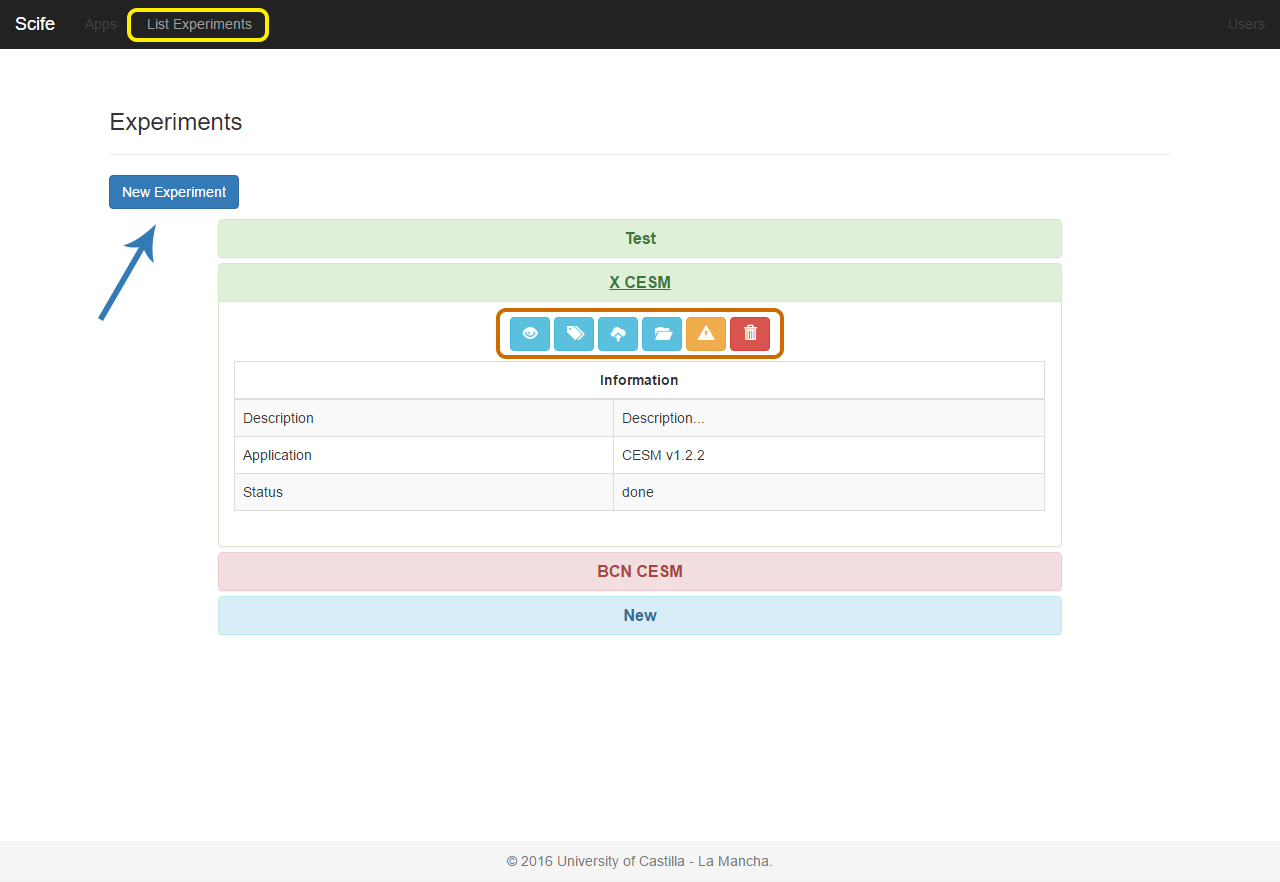
\includegraphics[width=\linewidth]{index}
	\caption{Experiment index view.}
	\label{fig:index}
\end{figure}

When you deploy an experiment, you will see some info and buttons. For example, the Figure \ref{fig:index} shows the ``X CESM'' experiment deployed with the next information:
\begin{itemize}
	\item Description: in this field the user will see the the info inserted when the experiment was created.
	\item Application: this field shows the name of the application associated with the experiment. In this case ``CESM v.1.2.2''
	\item Status: finally, the user can see the status of the experiment, besides of the colour bar.
\end{itemize}

You can also see a series of buttons in each experiment (see Figure \ref{fig:index} marked in orange colour). This buttons allow the user browse the application functions of the experiment in question:
%todo Completar cada boton con la referencia a cada sección
\begin{itemize}
	\item The first button (eye open) redirect the user to the overview view, learn more in Section \ref{sec:overview}.
	\item The second button redirects the user to the labels view, see in Section \ref{sec:labels}.
	\item The next button opens a new view that allows the user upload files to experiment, see more in Section \ref{sec:inputData}.
	\item The button with a open folder redirects the user to sources view, see in Section \ref{sec:sources}.
	\item The yellow button redirects the user to the logs view (Section \ref{sec:logs}).
	\item Finally, the red button with a trash allows the user delete an experiment. When you click this button, a modal view appear to confirm the user action as you can se in the Figure \ref{fig:index-delete}. 
\end{itemize}

\begin{figure}[htp]
\centering
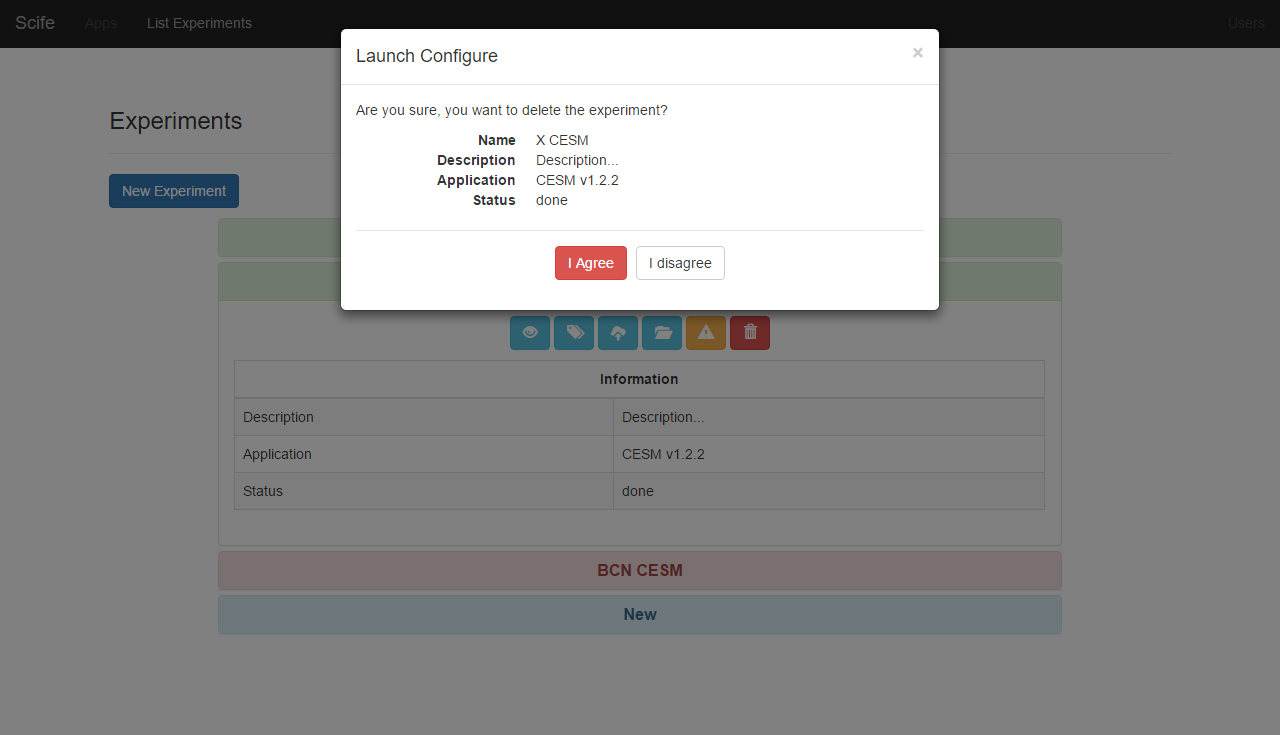
\includegraphics[width=\linewidth]{img/index-delete}
\caption{Modal view to confirm the deletion experiment.}
\label{fig:index-delete}
\end{figure}

From the index view, you can create new experiments, only have to click the ``\texttt{New Experiment}'' button. After that, a new view will appear, like the shown in the Figure \ref{fig:create}. You need input some information to create the new experiment like its name, description or the application in which the experiment will be executed.
\begin{figure}[htp]
	\centering
	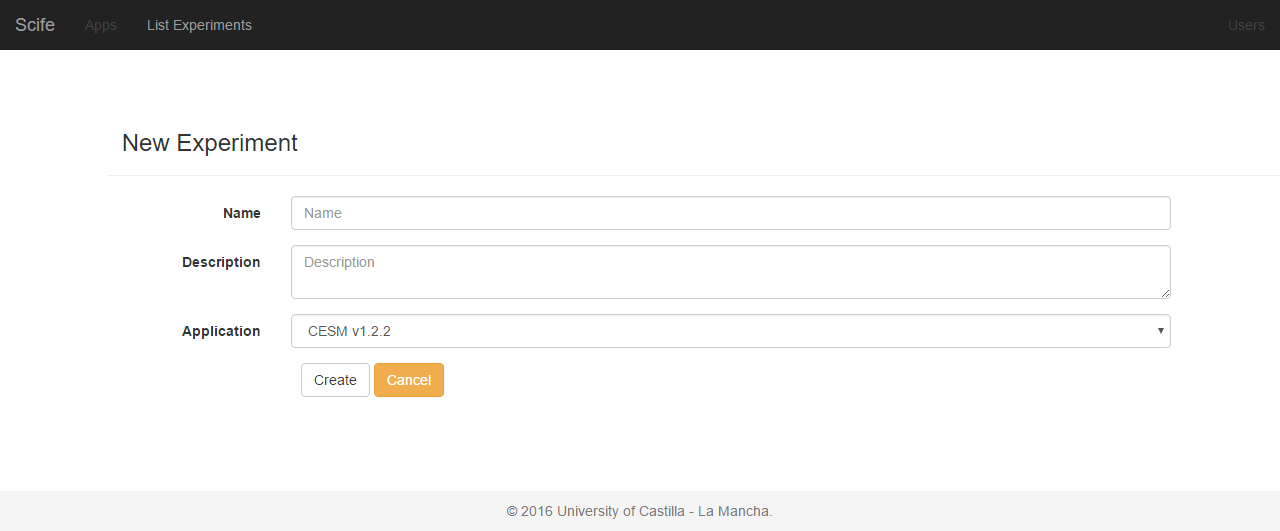
\includegraphics[width=\linewidth]{img/create}
	\caption{View with the form to create a new experiment.}
	\label{fig:create}
\end{figure}

\subsection{Overview}\label{sec:overview}
The overview is the main view of an experiment, in this page you can launch, reset, delete the experiment or download the results when the execution has finished. See the Figure \ref{fig:overview-done} as example, notice the buttons in the centre of the page:
\begin{figure}[htp]
	\centering
	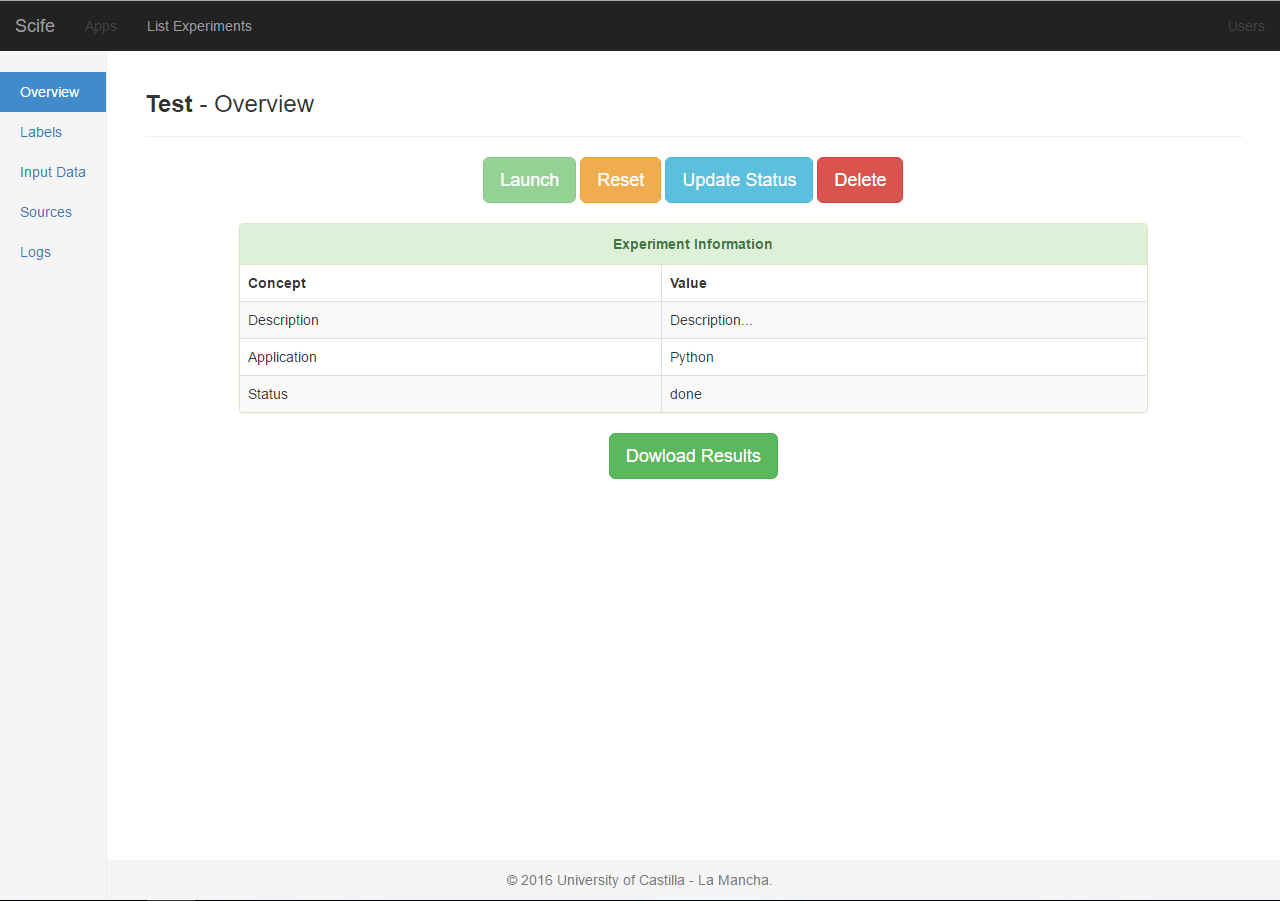
\includegraphics[width=\linewidth]{img/overview-done}
	\caption{The overview view.}
	\label{fig:overview-done}
\end{figure}

\begin{itemize}
	\item Launch button, allow the user execute the experiment. This button only is available when the experiment status is ``created''. When you click this button, the launch modal view will appear, as you can se in the Figura \ref{fig:overview-launch}. In the launch modal you must select the number of nodes, the image and the size of each node where the experiment will be executed. Besides, in the bottom of the modal, you will see information about the cluster where you will execute the experiment, ``Fedora Science'' in this case.
	\item The reset button allows the user stop the experiment execution.
	\item With the ``Update Status'' you can refresh the experiment status to known its status (launched, failed, done, etc.).
	\item Finally, the ``Delete'' button allows delete the experiment. Before do that, appear a modal view to confirm the deletion as you can see in the Figure \ref{fig:overview-delete}.
\end{itemize}

\begin{figure}[htp]
	\centering
	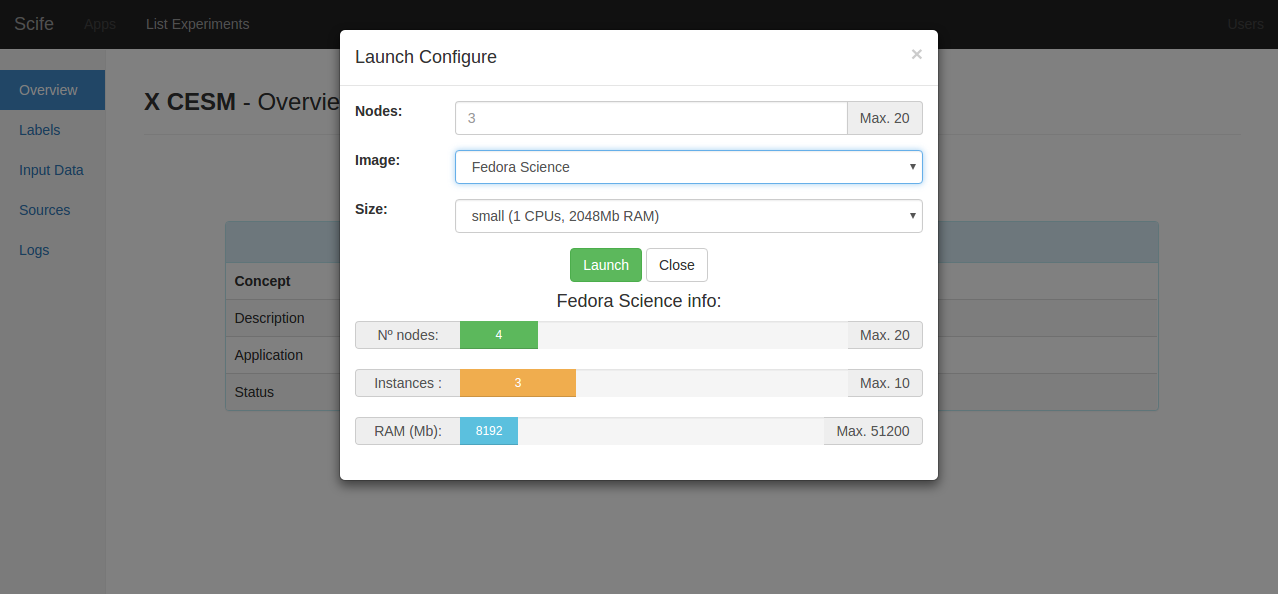
\includegraphics[width=\linewidth]{img/overview-launch}
	\caption{The launch modal view in the overview page.}
	\label{fig:overview-launch}
\end{figure}
\begin{figure}[htp]
	\centering
	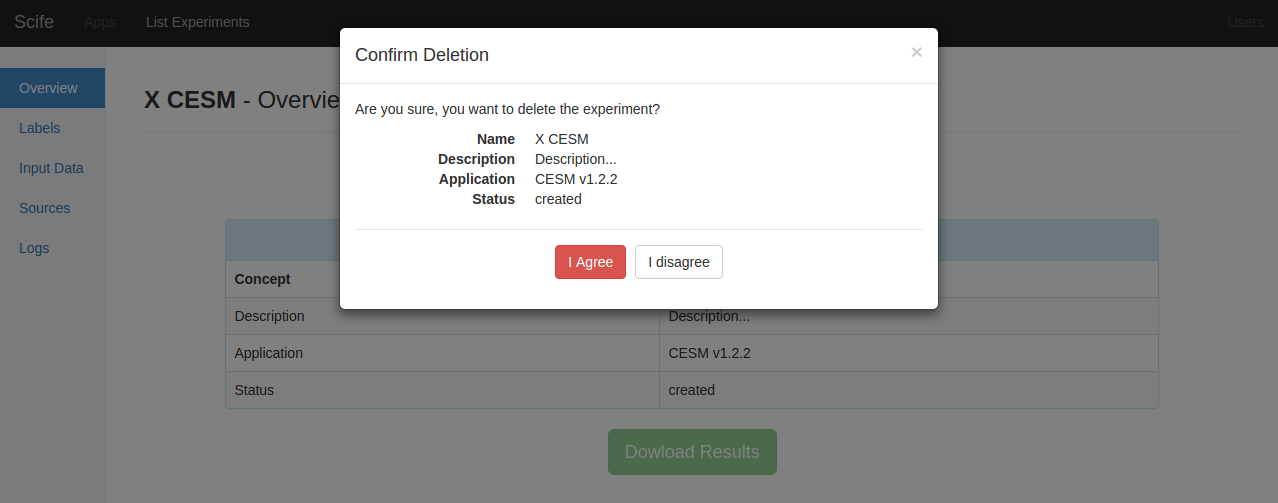
\includegraphics[width=\linewidth]{img/overview-delete}
	\caption{Confirm deletion modal view in the overview page.}
	\label{fig:overview-delete}
\end{figure}

\subsection{Labels}\label{sec:labels}
In this page, you can add, edit and delete the labels associate with an experiment. In the Figure \ref{fig:labels} you can see the view shown the user to modify the labels. When you open this window, the application shows the current labels in the experiment. For example, in the Figure \ref{fig:labels} the ``\texttt{COMPSET}'' label is set to ``\texttt{X}'' or the ``\texttt{GRID\_RESOLUTION}'' label to ``\texttt{t19\_g16}''.
\begin{figure}[htp]
	\centering
	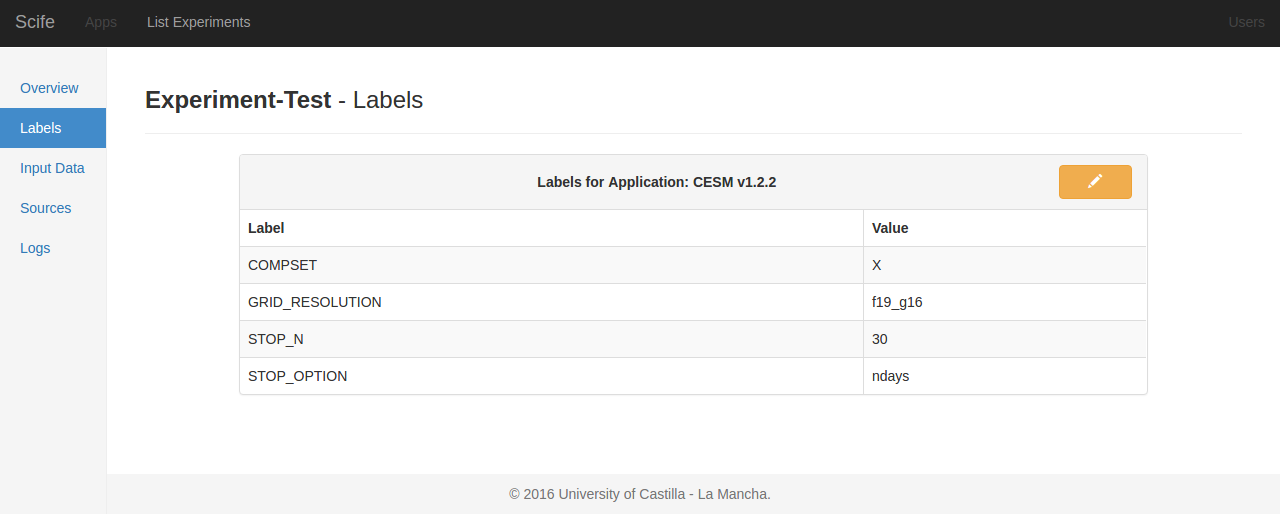
\includegraphics[width=\linewidth]{img/labels}
	\caption{Labels page of an experiment.}
	\label{fig:labels}
\end{figure}

If you want update (add, edit or delete) the labels, only have to click the top-right yellow button which contains a pen icon. When you click this button a new form will be deploy as you can see in the Figure \ref{fig:labels-edit}. Available labels will be shown in this form:
\begin{itemize}
	\item If you want add a new value to a label, only have to put the value you want in the label.
	\item If you want edit the value of a label, you have to modify the current value shown in the form.
	\item Finally, if you want delete a label, leave the field empty.
\end{itemize}

\begin{figure}[htp]
	\centering
	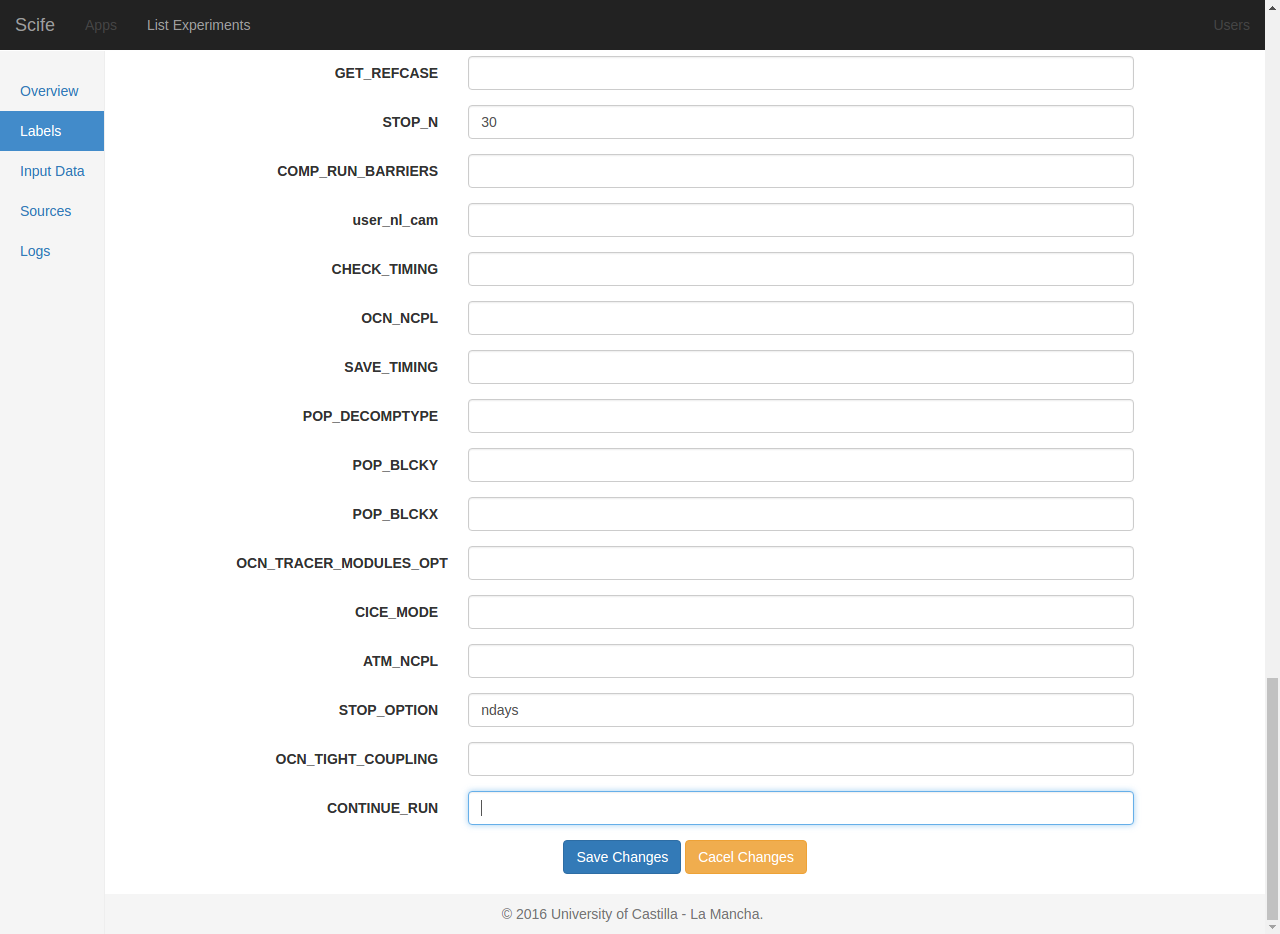
\includegraphics[width=\linewidth]{img/labels-edit}
	\caption{Form to edit the labels of an experiment page.}
	\label{fig:labels-edit}
\end{figure}

\subsection{Input data}\label{sec:inputData}
In this view, you can upload files to the cloud associated with the experiment. The view will be similar to that shown in the Figure \ref{fig:input-data} which is divided in two main parts.\\
\begin{figure}[htp]
	\centering
	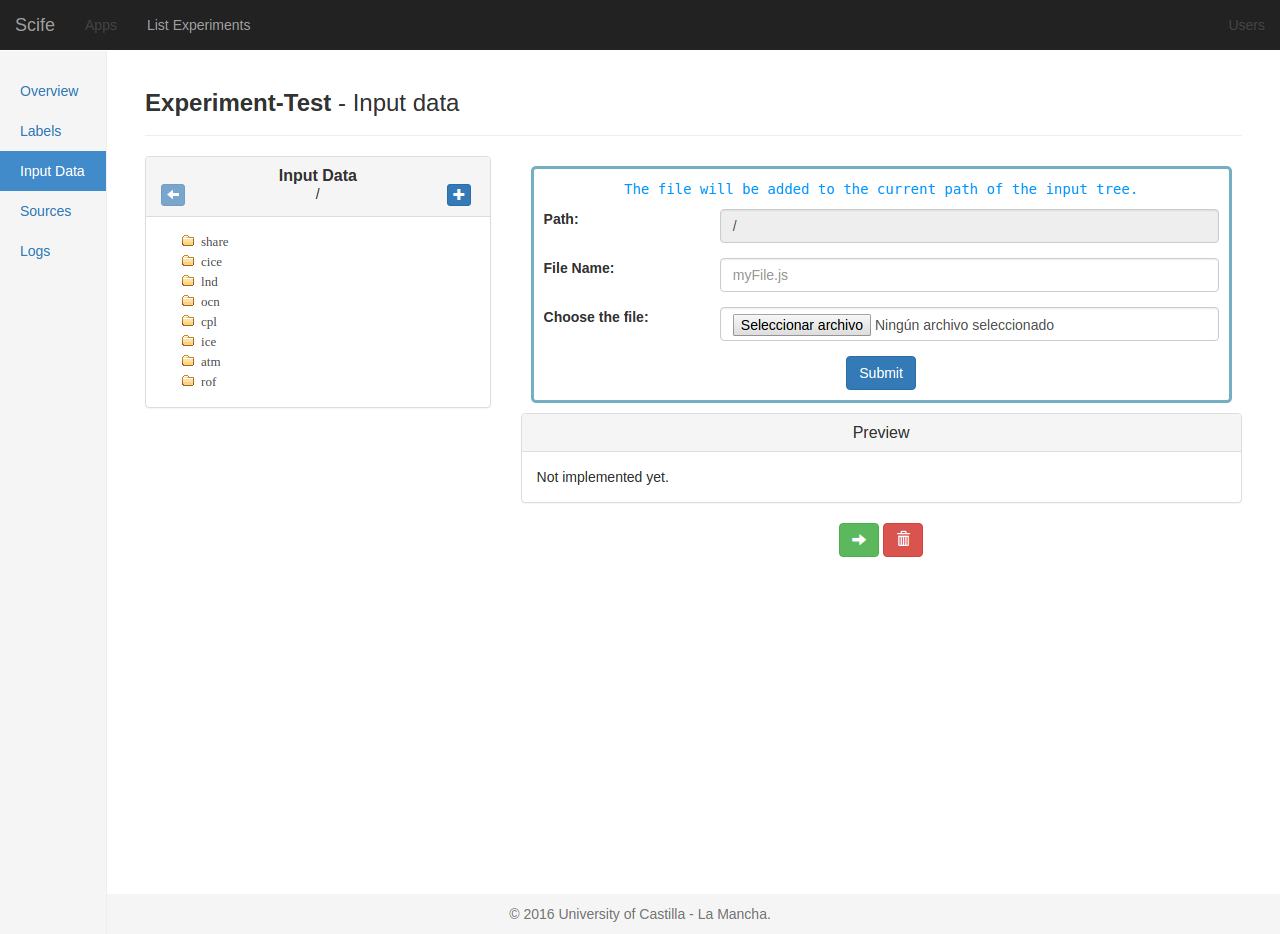
\includegraphics[width=\linewidth]{img/input-data}
	\caption{Input data view of an experiment.}
	\label{fig:input-data}
\end{figure}

In the left side, you can se a tree with the files and folders you have in the cloud. When you click in a folder a new tree view will appear with the contains of the folder clicked. When you enter in a folder, you can return to the parent folder with the button marked with in green colour. When you are in the root folder ``/'' this button will be disabled. If you want create a new folder, you can make it clicking in the button marked in red colour. When you click this button, a new modal view will be shown like the Figure \ref{fig:input-create-folder}. In this modal you will see the path where the folder will be created and you need set the name to the new folder.
\begin{figure}[htp]
	\centering
	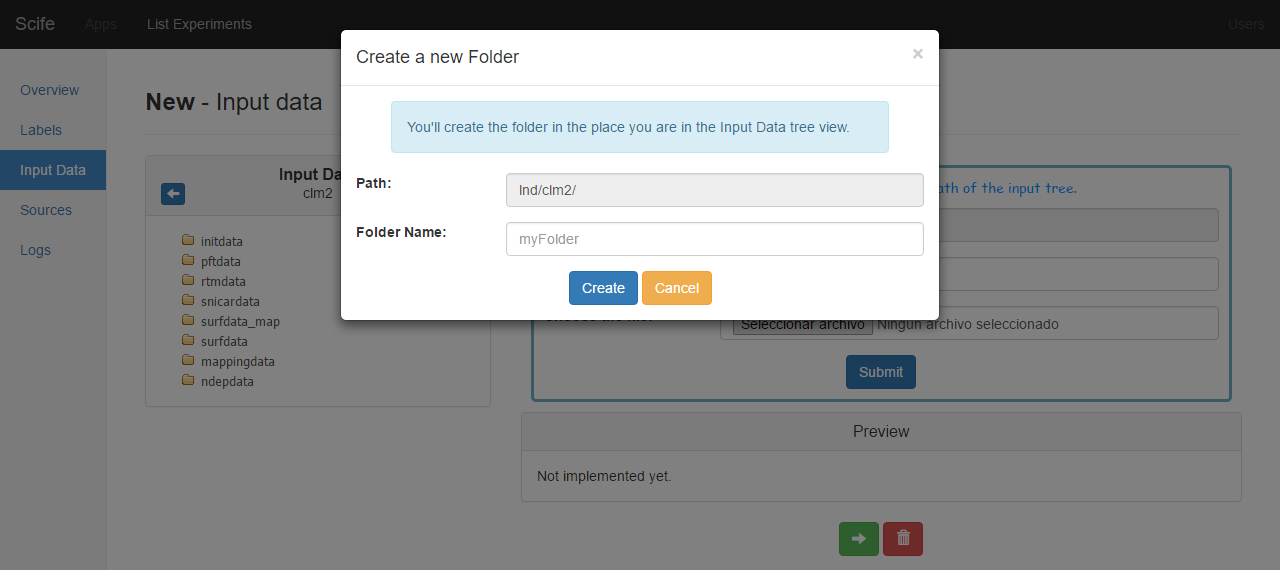
\includegraphics[width=\linewidth]{img/input-create-folder}
	\caption{Modal view to create a new folder in the input data view.}
	\label{fig:input-create-folder}
\end{figure}

In the right side of the Figure \ref{fig:input-data} (blue rectangle) are a form where you can upload a file in the current folder of the tree view. Besides, in the ``\texttt{Path}'' label you will see the path where the file will be uploaded.

\subsection{Sources}\label{sec:sources}
This page allows the user edit the files of the an experiment. The aspect of this view is like the Figure \ref{fig:sources}. In the left side, similar to input data view, you can browser the source files and folder. If you click a folder the tree view will show the contains of the folder selected, but if you click a file the contains of the file will be shown in the code editor (right-side). In the sources tree view you can create a new folder, you can make it clicking the button marked with green colour and a modal view like the Figure \ref{fig:input-create-folder} will appear.\\
\begin{figure}[htp]
	\centering
	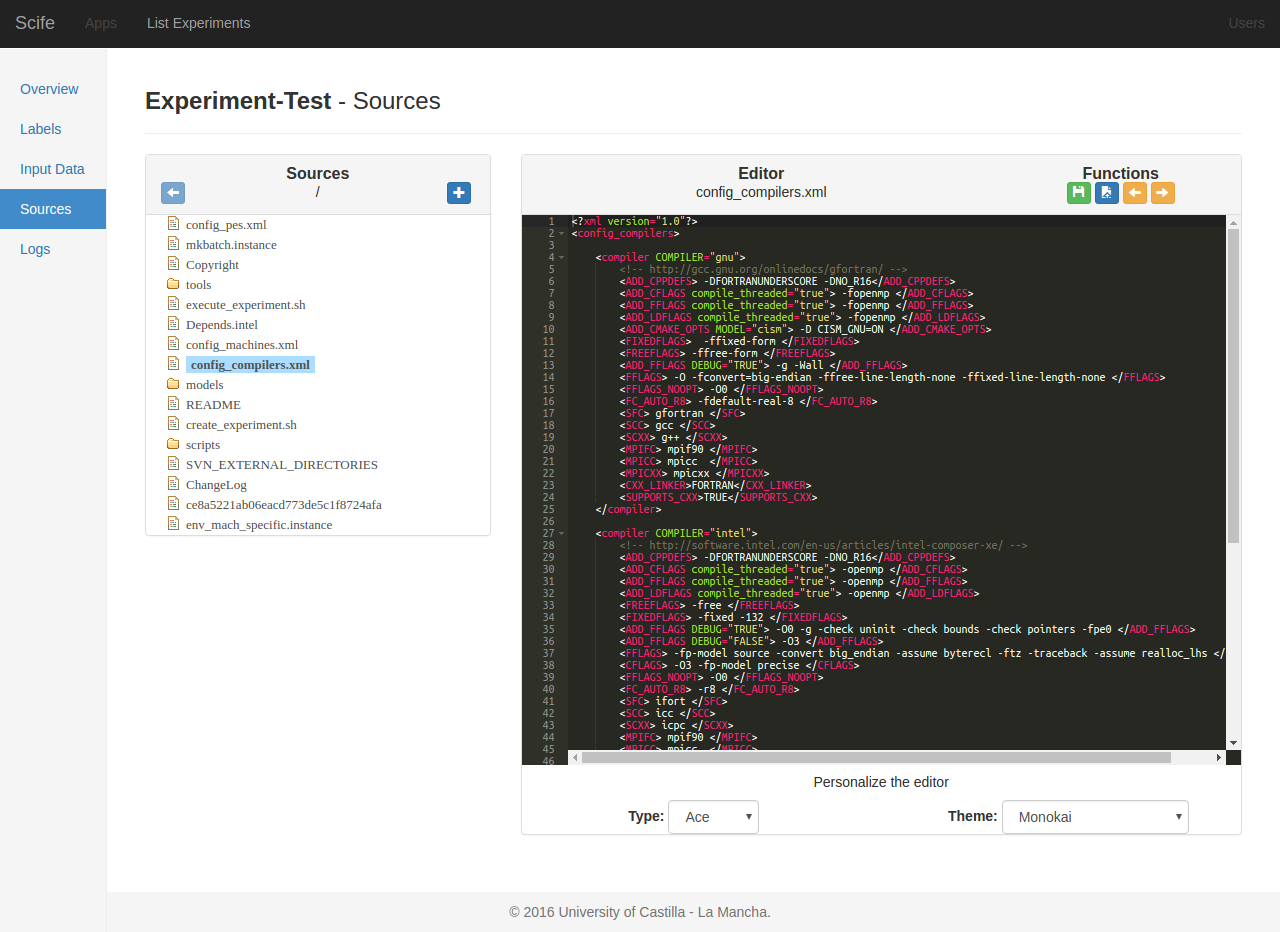
\includegraphics[width=\linewidth]{img/sources}
	\caption{Sources view of an experiment.}
	\label{fig:sources}
\end{figure}

When you select a file, its contain will appear in the code editor where you can edit it. At the bottom of the code editor you can personalize it, modifying the editor type (ace, vim or emacs) or select a theme from the long list. In the top-right side of the editor are four buttons with the next functions:
\begin{itemize}
	\item The first button in green colour allows the user save the changes made in the file.
	\item The second blue button allows the user create a new file with the current information of the editor. When you click this button a modal view will be shown (Figure \ref{fig:sources-new-file}) where you need name the new file, and will see the path where the file will be created.
	\item The next button with a left arrow undo the changes made in the editor.
	\item The latest button with a right arrow redo the changes.
\end{itemize}
\begin{figure}[htp]
	\centering
	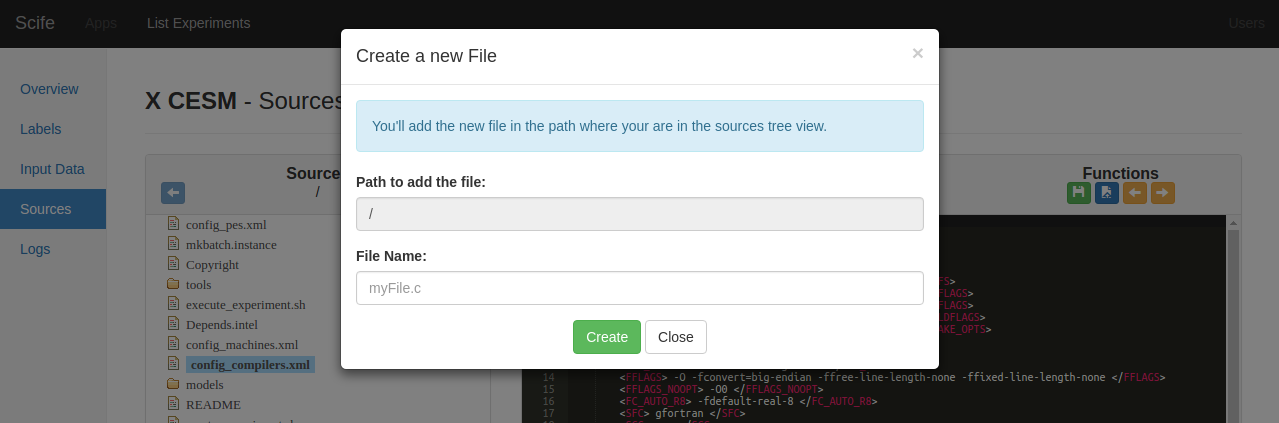
\includegraphics[width=\linewidth]{img/sources-new-file}
	\caption{Modal view to create a new file in the sources view.}
	\label{fig:sources-new-file}
\end{figure}

\subsection{Logs}\label{sec:logs}
When you launch an experiment the logs will be shown in this view. The Figure \ref{fig:logs-listed} shows an example of this view. In this view the selection list contains a list with the logs file names, when you select one its contain will appear in the window.
\begin{figure}[htp]
	\centering
	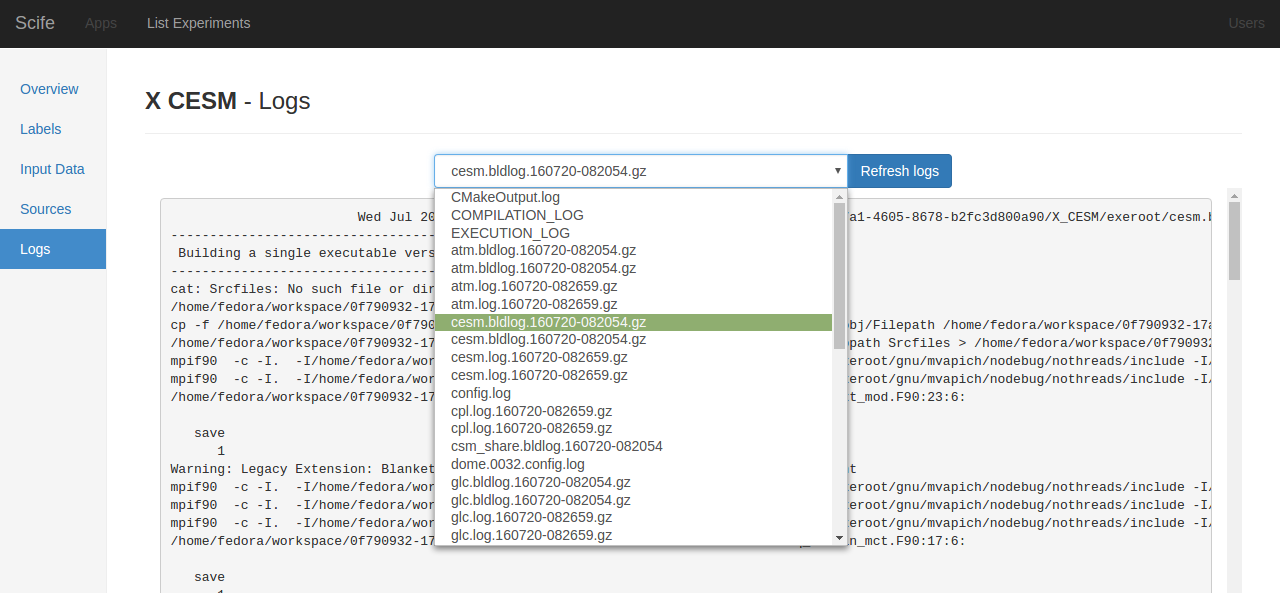
\includegraphics[width=\linewidth]{img/logs-listed}
	\caption{Sources view of an experiment.}
	\label{fig:logs-listed}
\end{figure}

\end{document}
